\subsection{$B_s$-Mixing}
\begin{figure}[t]
 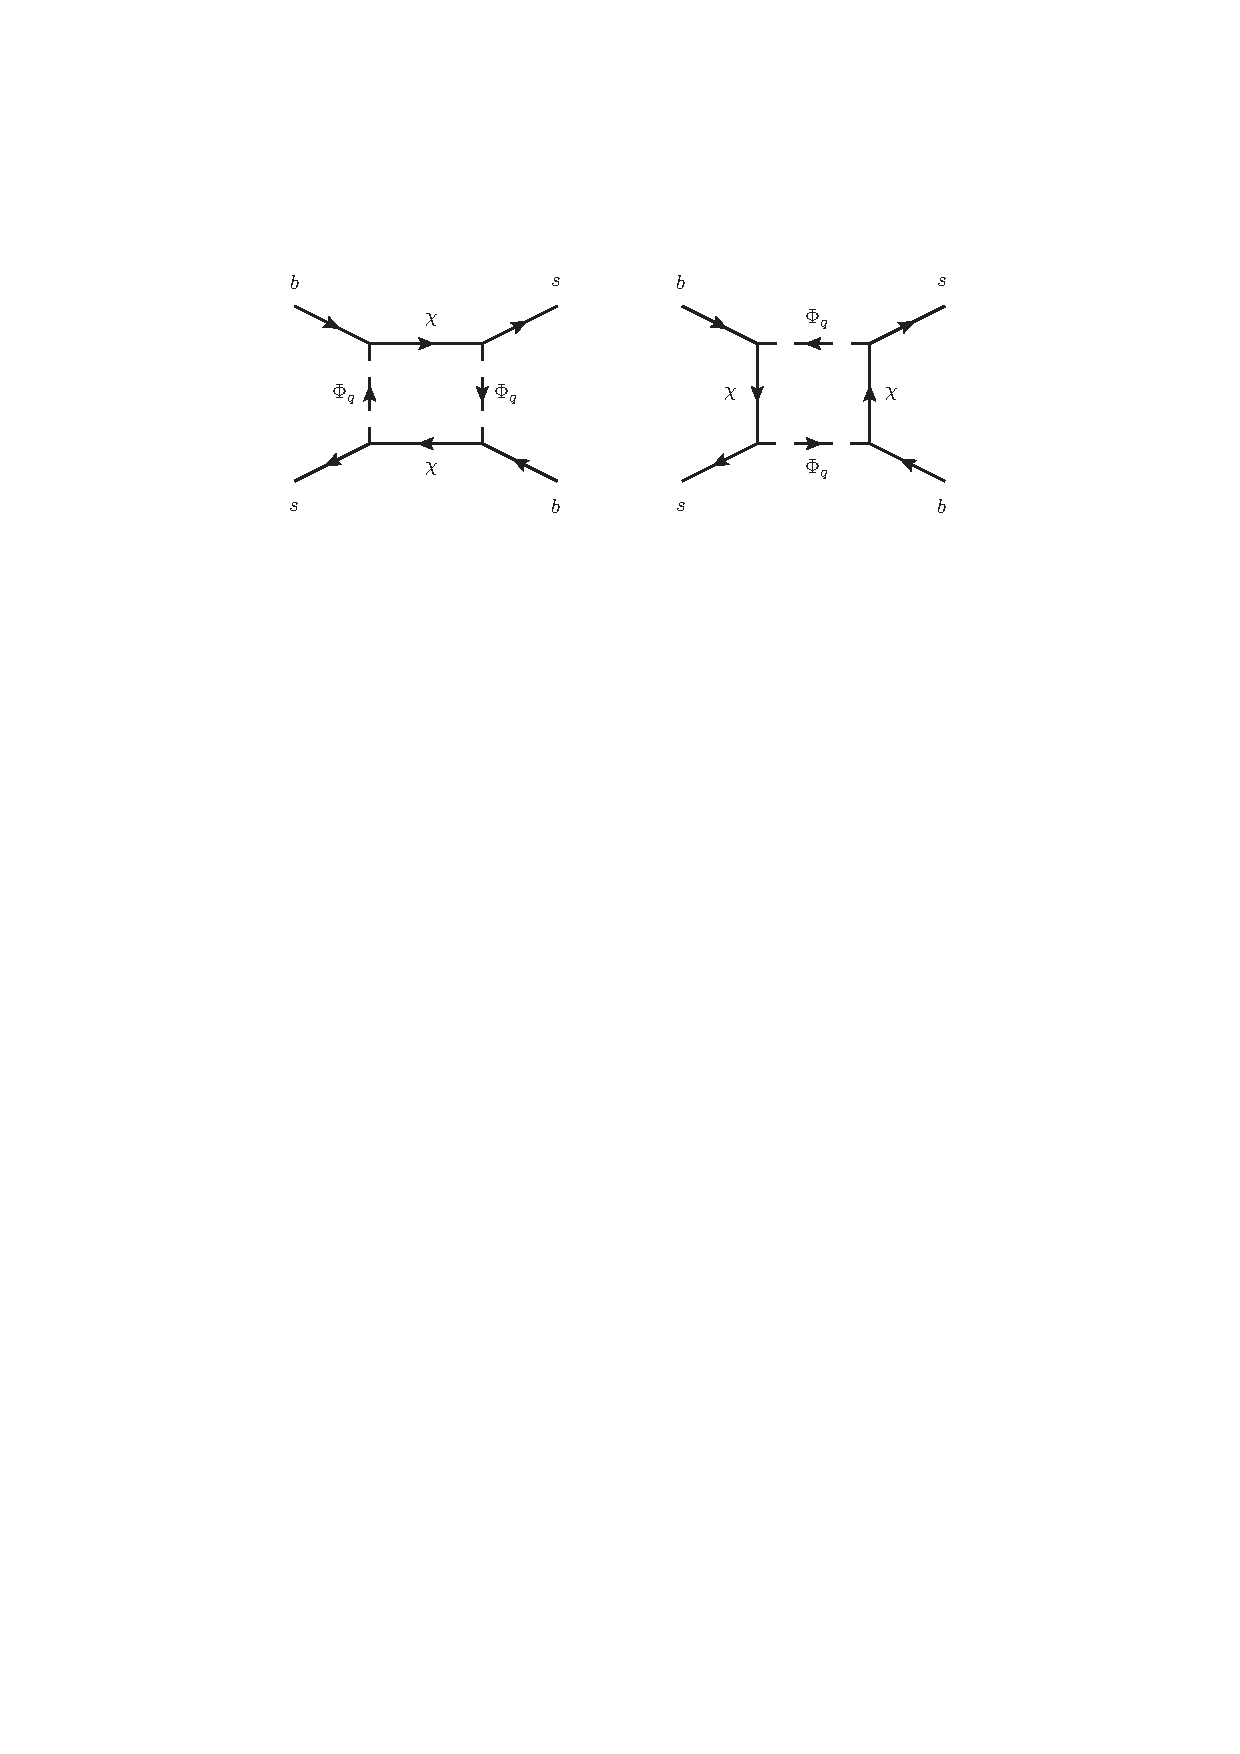
\includegraphics[width=0.6\textwidth]{../pics/bsmix.pdf}
 \caption{$B_s$-mixing. The crossed boxes also occur, see fig. \ref{pic_Bsmumu}}
 \label{pic_Bsmix}
\end{figure}
When there are semileptonic meson decays, hadronic ones are accordingly enabled. The diagrams for $B_s$-mixing are depicted in figure \ref{pic_Bsmix}. Other
meson mixings like $K\bar K$ or $ D \bar D$ are suppressed due to their smaller Yukawa couplings. From a calculational point of view, this process is 
quite similar to the former $B_s\rightarrow \mu\mu$ and is induced only through one-loop box diagrams in the SM to lowest order. The effective Hamiltonian
involves only one operator $(\bar s \gamma^\mu P_L b)(\bar s \gamma_\mu P_L b)$ for our chiral theory whose Wilson coefficient reads
\begin{align}
 C_{B\bar B}^A &=  \frac{|g_2^{q*}g_3^q|^2}{m^2} \frac{1}{128\pi^2} \left(K'(x_q) + G'(x_q)\right)\\
 C_{B\bar B}^B &=  \frac{|g_2^{q*}g_3^q|^2}{m^2} \frac{5}{384\pi^2} \left(K'(x_q) + \frac15 G'(x_q)\right)
\end{align}
with the first derivatives $K'(x)$ and $G'(x)$. 

